\documentclass{article}

\usepackage[preprint]{neurips_2023}

\usepackage[utf8]{inputenc} % allow utf-8 input
\usepackage[T1]{fontenc}    % use 8-bit T1 fonts
\usepackage{hyperref}       % hyperlinks
\usepackage{url}            % simple URL typesetting
\usepackage{booktabs}       % professional-quality tables
\usepackage{amsfonts}       % blackboard math symbols
\usepackage{nicefrac}       % compact symbols for 1/2, etc.
\usepackage{microtype}      % microtypography
\usepackage{xcolor}         % colors
% \usepackage[colorlinks]{hyperref}
\usepackage[nameinlink,noabbrev]{cleveref}
\crefformat{figure}{\textsuperscript{#2#1#3}}
\crefformat{table}{\textsuperscript{#2#1#3}}
\usepackage{titlesec}

\setcounter{secnumdepth}{4}

\titleformat{\paragraph}
{\normalfont\normalsize\bfseries}{\theparagraph}{1em}{}
\titlespacing*{\paragraph}
{0pt}{3.25ex plus 1ex minus .2ex}{1.5ex plus .2ex}


\title{Exceedingly Simple Handwritten Digit Classifier}

\author{
	Brandon Szeto \thanks{160 lbs} \\
	Jacobs School of Engineering \\
	University of California, San Diego \\
	San Diego, CA 92122 \\
	\texttt{bszeto@ucsd.edu} \\
	\AND
	Nathaniel Thomas \thanks{200 lbs} \\
	Jacobs School of Engineering \\
	University of California, San Diego \\
	San Diego, CA 92122 \\
	\texttt{nathomas@ucsd.edu} \\
}

\begin{document}

\maketitle

\begin{abstract}
	The paper explores backpropagation, employing numerical approximation to verify accuracy. It introduces momentum in stochastic gradient descent, demonstrating its impact on model convergence and the trade-off with slight performance penalty. The study delves into regularization experiments (L1, L2) and observes the trade-off between convergence speed and accuracy. Activation function experiments (tanh, sigmoid, ReLU) highlight their impact on test accuracy and convergence speed, with tanh outperforming others in terms of both accuracy and speed. Adjusting learning rates addresses issues with ReLU's initial high rate. We also display the most difficult to classify digits. Overall, the findings contribute insights into optimizing neural networks.
	% This paper explores various methods for handwritten digit classification using the MNIST dataset. The dataset is split, normalized, and subjected to softmax regression, backpropagation, momentum, early stopping, and regularization techniques. Activation functions (tanh, sigmoid, ReLU) are evaluated. The study reveals trade-offs between convergence speed and accuracy, contributing insights into neural network training for digit classification.
\end{abstract}


\begin{figure}[!h]
	\centering
	
\includegraphics[width=0.25\textwidth]{./images/mnist_digit.png}
	\caption{Sample MNIST Digit (5)}
	\label{fig:example}
\end{figure}


\section{Data Loading}
The dataset we will be using to train a multi-layer neural network is the
MNIST dataset. The {MNIST}\footnote{\textit{Modified} National Institute of
	Standards and Technology} dataset is a collection of grayscale handwritten
digits commonly used for training various image processing systems. The dataset
contains 60,000 training images and 10,000 testing images each normalized to $28
	\times 28$ pixels.

\subsection{Data Splitting}
The MNIST dataset is split using an 80-20 ratio. Since the MNIST dataset
contains 60,000 training images and 10,000 testing images, we expect to have
48,000 images and target labels in the training set and 12,000 images and
target labels in the validation set. Optionally, the dataset is randomly
shuffled and seeded for reproducability.

\subsection{Normalization}
The training and validation datasets are normalized by z-score.

$$ \vec{z} = \frac{\vec{x} - \mu}{\sigma} $$

Here, $\vec{x}$ is the flattened ($ 28 \times 28 = 784$) vector, $\mu$ is
the mean pixel value, and $\sigma$ is the standard deviation over the single
image. The resulting vector $\vec{z}$ (also size $784$) contains the z-score
normalization of the image where each value will range between -1 and 1 (unit
variance) and have mean 0.

\subsection{Mean and Standard Deviation}
Consider an image of the digit $5$\cref{fig:example}. Its vector representation is

\begin{equation*}
	\vec{x}^{(n)}  =
	\begin{bmatrix}
		x_1    \\
		x_2    \\
		\vdots \\
		x_n
	\end{bmatrix}
\end{equation*}

where each of the values in $\vec{x}^{(784)}$ is some value between 0 for black
and 255 for white. Its mean ($\mu$) and standard deviation ($\sigma$) can be
obtained by

\begin{equation*}
	\begin{aligned}
		\mu    & = \frac{x_1 + x_2 + \ldots + x_n}{n}            & = 0.13714225924744897 \\
		\sigma & = \sqrt{\frac{\sum_{i=1}^{n} (x_i - \mu)^2}{n}} & = 0.31112823799846606
	\end{aligned}
\end{equation*}

These values can then be used to obtain $\vec{z}^{(n)}$, the z-score
normalization of $\vec{x}^{(n)}$.


\section{Softmax Regression}

\subsection{Background}
Firstly, we perform softmax regression on a single-layer neural network (i.e.
input layer directly connects to output layer). Given an input $x^{(n)}$ and $c$
possible classes, softmax regression will output a vector $y^{(n)}$, where each
element, $y^{(n)}_k$ represents the probability that $x^{(n)}$ is in class $k$.

\begin{equation*}
	\begin{aligned}
		y^{(n)}_k & = \text{softmax}(a^{(n)}_k)_ =
		\frac{e^{a^{(n)}_k}}{\sum_{j=1}^{N} e^{a^{(n)}_j}} \\
		a^{(n)}_k & = w^\top_k x^{(n)}
	\end{aligned}
\end{equation*}

Here, the softmax activation function generalizes the logistic activation
function for multiple classes. Now for \textit{softmax regression}, we use a
one-hot encoding for our targets. Together, we can calculate loss via the
cross-entropy cost function defined as

\begin{equation*}
	E = - \sum_k \sum_{k = 1}^c t^{(n)}_k \ln \left( y^{(n)}_k \right)
\end{equation*}

and its corresponding gradient

\begin{equation*}
	-\frac{\partial E^n(w)}{\partial w_{j k}}=\left(t_k^{(n)}-y_k^{(n)}\right) x_j^n
\end{equation*}

The above equations can be combined to implement the following delta rule to
update the weights over each epoch.

\begin{equation*}
	\begin{aligned}
		\delta_j & = (t_j^{(n)}-y_j^{(n)})         & \text{ for output unit } j \\
		\delta_j & = g'(a_j)\sum_k \delta_k w_{jk} & \text{ for hidden unit } j
	\end{aligned}
\end{equation*}

In pseudocode, we have

\begin{algorithm}
	\caption{Stochastic Gradient Descent}
	\begin{algorithmic}
		\State $w \gets 0$
		\For{$t = 1$ to $M$}
		\State Randomize the order of the indices into the training set
		\For{$j = 1$ to $N$ in steps of B}
		\State start = $j$
		\State end = $j$ + B
		\State $w_{t + 1} = w_t - \alpha \sum_{n = \text{start}}^{end} \nabla
			E^{(n)}(w) $
		\EndFor
		\EndFor
	\end{algorithmic}
\end{algorithm}

\subsection{Performance}

In a single layer neural network as defined in \texttt{./config\_4.yaml}, we
obtain the following results using softmax regression over 100 epochs. Below we
plot loss versus epochs~\ref{fig:loss} and accuracy versus epochs~\ref{fig:acc}.

\begin{figure}[ht]
	\centering
	\label{fig:loss}
	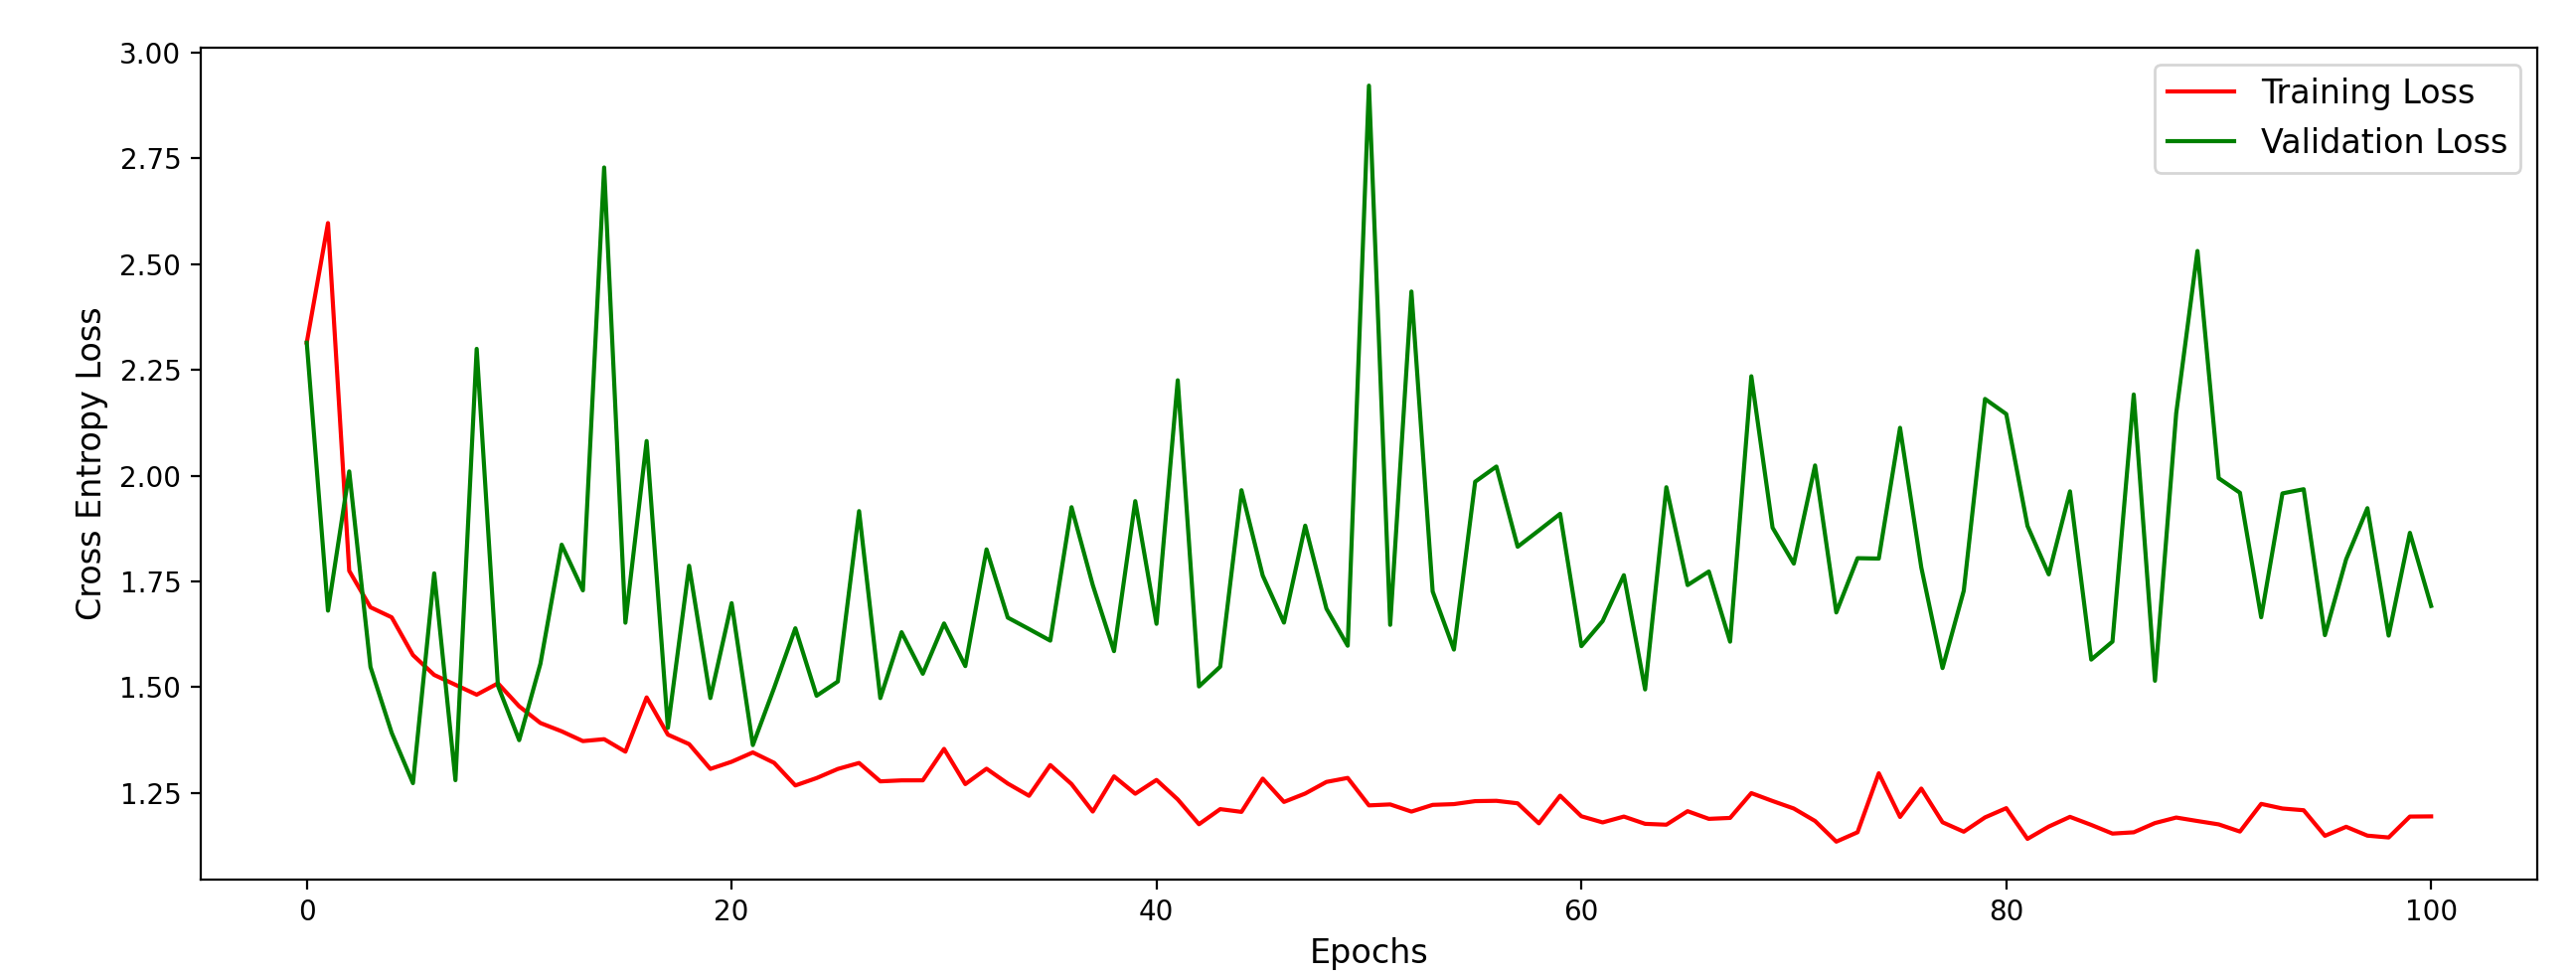
\includegraphics[width=1.0\textwidth]{./images/loss.png}
	\caption{Training/Validation Loss/Accuracy over 100 Epochs}
\end{figure}

\begin{figure}[!ht]
	\centering
	\label{fig:acc}
	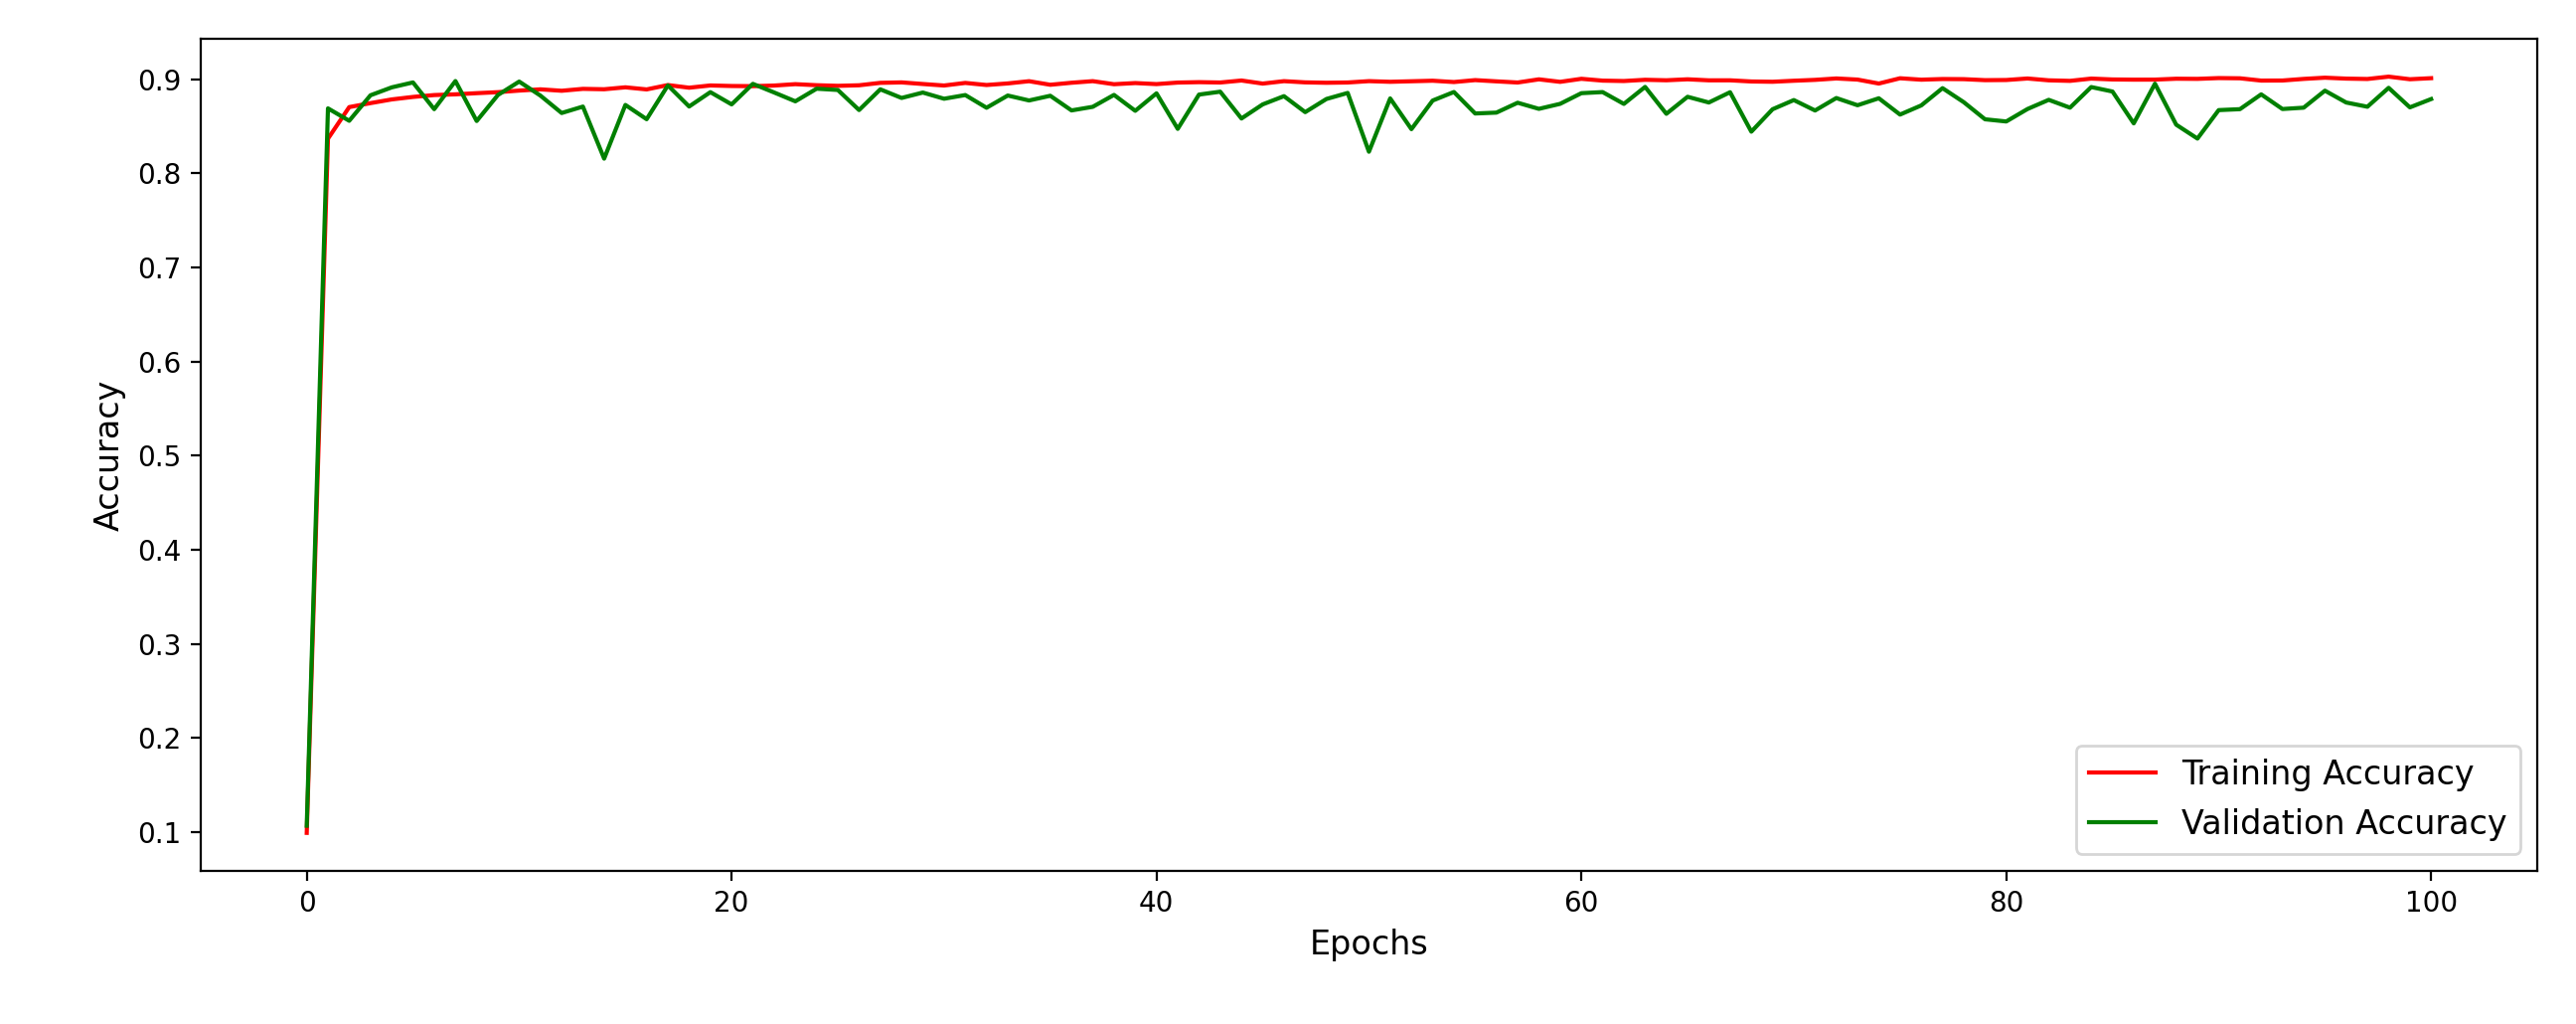
\includegraphics[width=1.0\textwidth]{./images/acc.png}
	\caption{Training/Validation Accuracy over 100 Epochs}
\end{figure}


\section{Backpropagation}


\section{Momentum Experiments}

\subsection{Background}

We now consider a new network with a 785 neuron input layer, a 128 neuron
hidden layer, and a 10 neuron output layer. The hidden layer is activated by
$\tanh(\mathbf x)$ and the output with softmax. We are training for 100 epochs.

Next, we implement momentum, which inserts inertia into the movement of the weights.
Instead of the weights being updated after each batch by

\begin{align*}
	w_{t + 1} = w_t - \alpha \sum_{n = \text{start}}^{end} \nabla E^{(n)}(w)
\end{align*}

we introduce the following \textit{velocity} term $v$.

\begin{align*}
	v_n = \gamma v_{n-1} - \alpha \nabla E^{(n)}(w)
\end{align*}

which is related to the weight update rule by

\begin{align*}
	w_{t+1} = w_t + v_B
\end{align*}


where $B$ is the batch size.

Along with momentum, we implement early stopping. This technique allows us
to stop training once performance stagnates on the validation set.


\begin{algorithm}
	\caption{Neural Network Training with Early Stopping}
	\begin{algorithmic}
		\State $TODO w \gets 0$
		% \For{$t = 1$ to $M$}
		% \State Randomize the order of the indices into the training set
		% \For{$j = 1$ to $N$ in steps of B}
		% \State start = $j$
		% \State end = $j$ + B
		% \State $w_{t + 1} = w_t - \alpha \sum_{n = \text{start}}^{end} \nabla
		% 	E^{(n)}(w) $
		% \EndFor
		% \EndFor
	\end{algorithmic}
\end{algorithm}


\subsection{Performance}

Without momentum, our training and validation plots look like this


\begin{align*}
	TODO
\end{align*}

Adding momentum, with $\gamma = 0.9$, our plots now look like this

\begin{figure}[!ht]
	\centering
	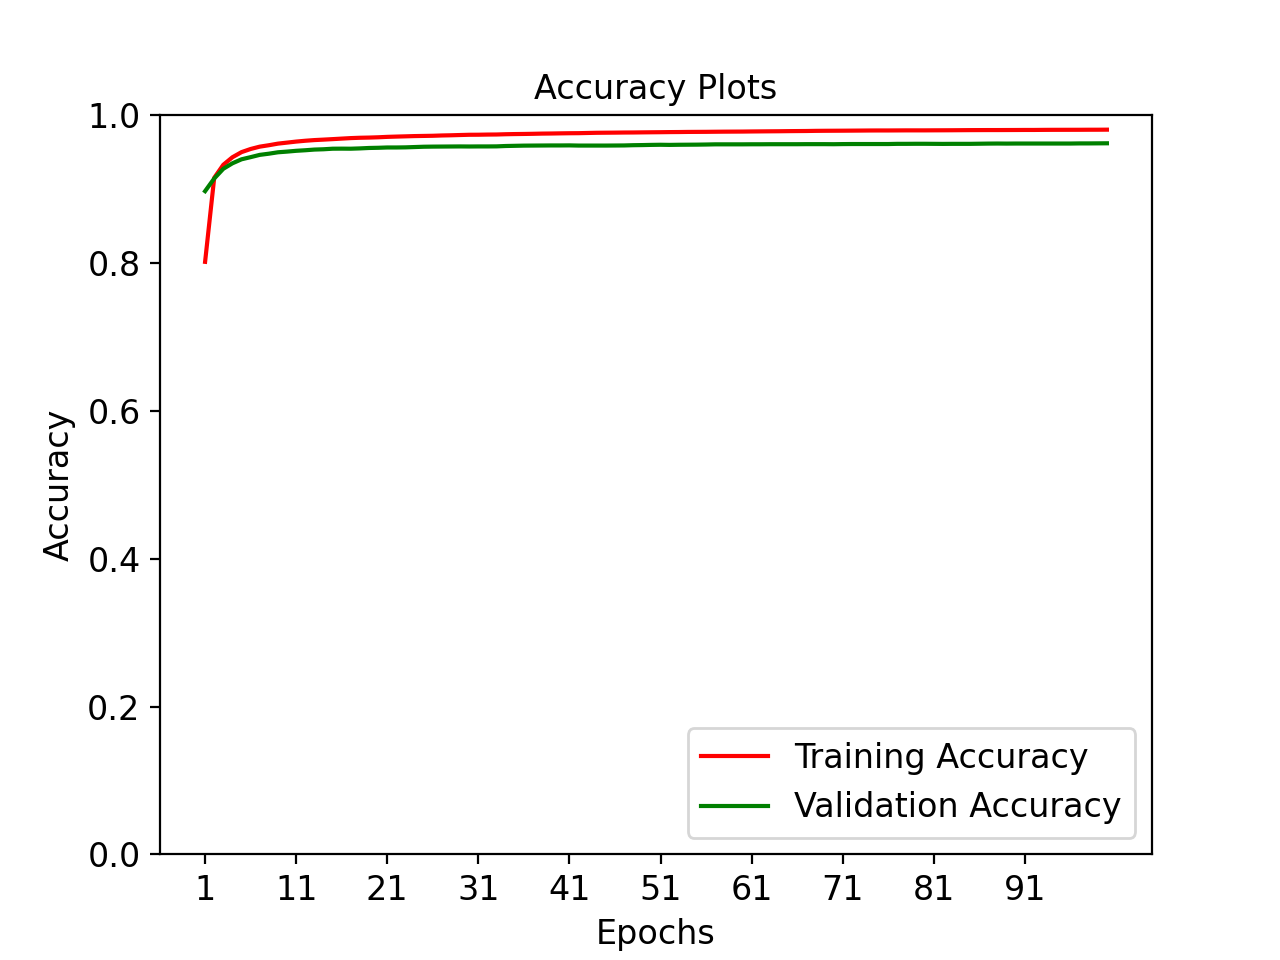
\includegraphics[width=1.0\textwidth]{./images/accuracy_momentum.png}
	\caption{Training/Validation accuracy with momentum over 100 Epochs}
\end{figure}

\begin{figure}[!ht]
	\centering
	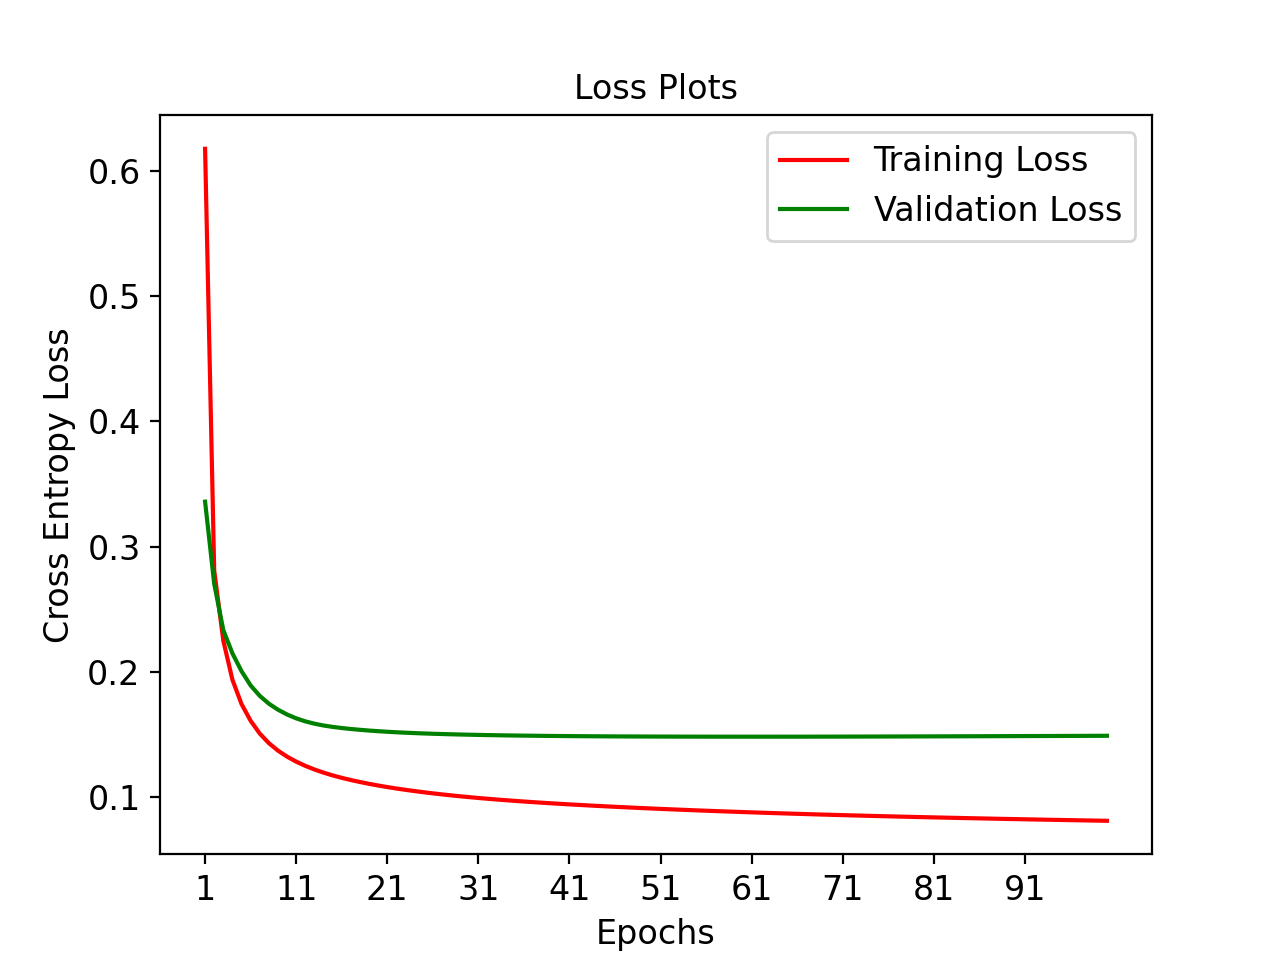
\includegraphics[width=1.0\textwidth]{./images/loss_momentum.png}
	\caption{Training/Validation loss with momentum over 100 Epochs}
\end{figure}

This model scores $96.64\%$ on the test set.


Next, we implement early stopping. We saw that 63 epochs were sufficient
for our training.

\begin{figure}[!ht]
	\centering
	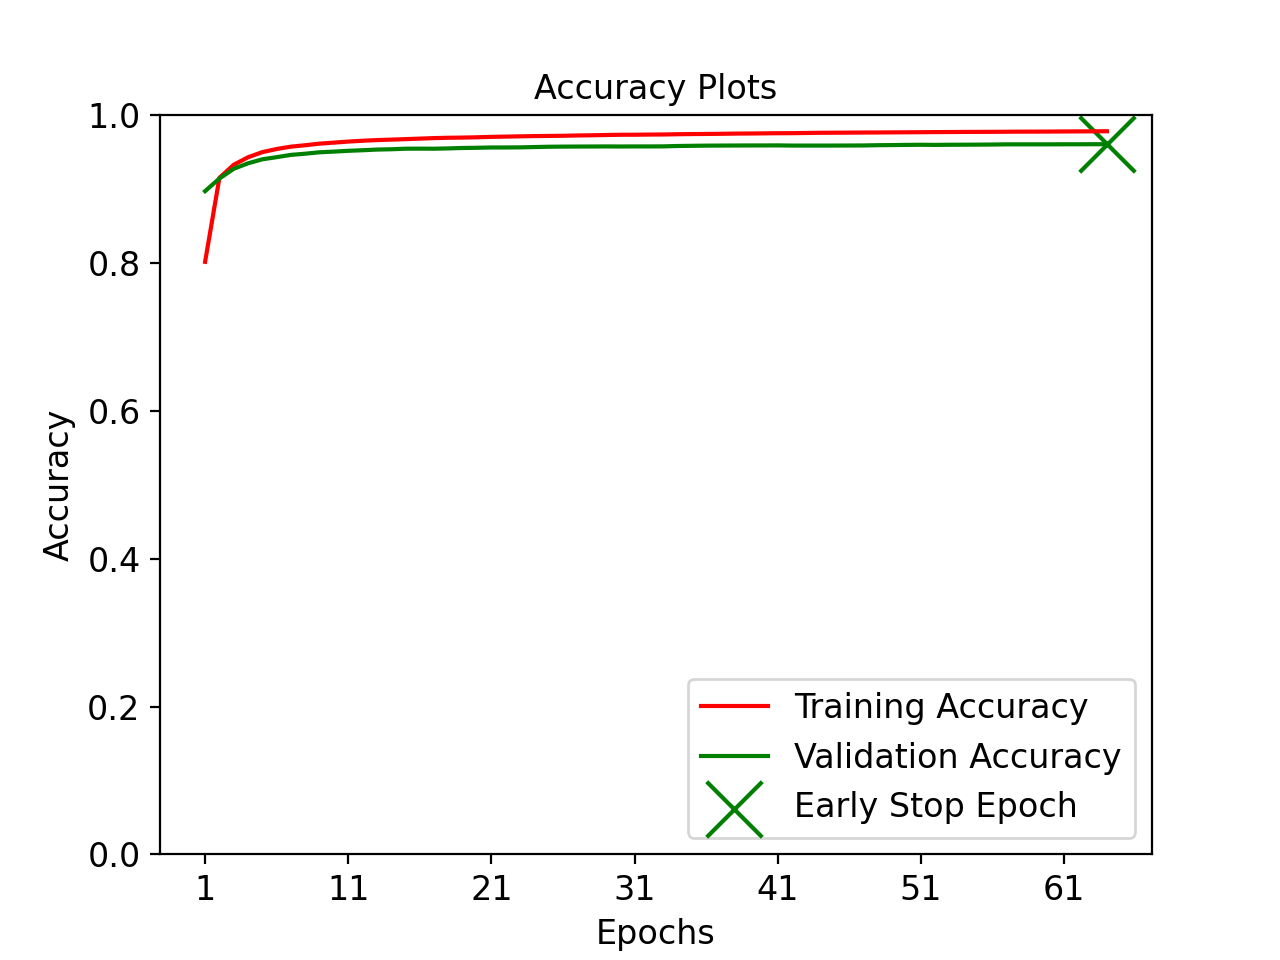
\includegraphics[width=1.0\textwidth]{./images/accuracy_momentum_early_stop.png}
	\caption{Training/Validation accuracy with momentum and early stopping}
\end{figure}

\begin{figure}[!ht]
	\centering
	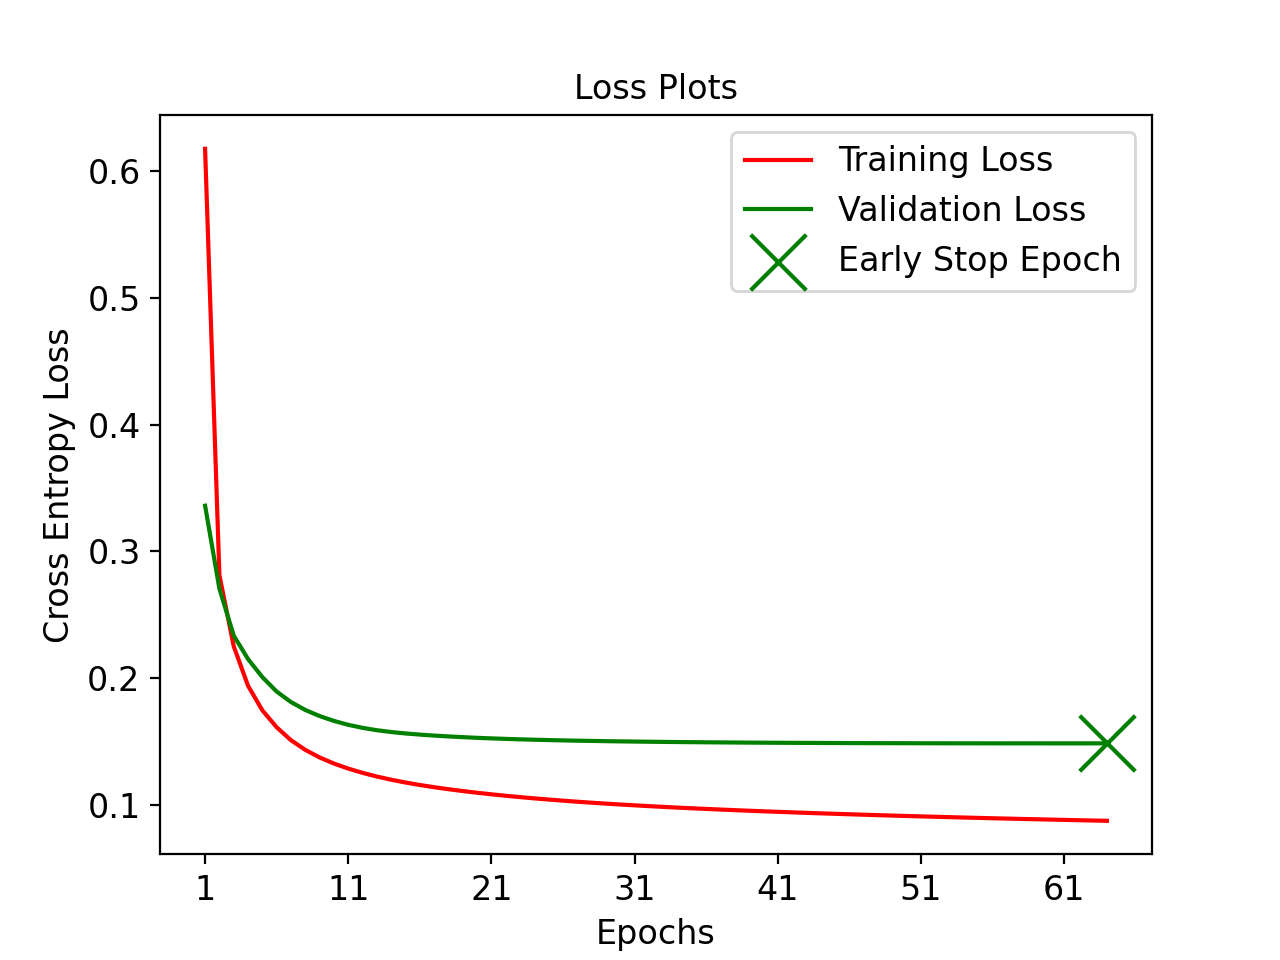
\includegraphics[width=1.0\textwidth]{./images/loss_momentum_early_stop.png}
	\caption{Training/Validation loss with momentum and early stopping}
\end{figure}

This model scores $96.56\%$ on the test set.

\subsection{Observations}

Momentum helps to smooth out noise in the gradients, especially when there are hidden layers. We also found
in testing that calculating $v$ within the batch performed significantly better than calculating $v$ after each
batch.

Early stopping is an excellent way to detect convergence, and saved us considerable training time. It also gives
an objective measure how many epochs are necessary for future training given a value of $\alpha$.


\section{Regularization Experiments}


\section{Activation Experiments}

\subsection{Background}

Neural networks utilize activation functions to introduce non-linearity into the model, enabling it to learn complex patterns and relationships in data. Three commonly used activation functions are \texttt{tanh}, \texttt{ReLU} (Rectified Linear Unit), and \texttt{sigmoid}.

\subsubsection{Tanh Activation Function}

The hyperbolic tangent function, \(\texttt{tanh}(x)\), is defined as:

\[
	\texttt{tanh}(x) = \frac{e^{x} - e^{-x}}{e^{x} + e^{-x}}
\]

The derivative of \(\texttt{tanh}(x)\) with respect to \(x\) is given by:

\[
	\frac{d}{dx} \texttt{tanh}(x) = 1 - \texttt{tanh}^2(x)
\]

Properties of \(\texttt{tanh}\):
\begin{itemize}
	\item Range: \([-1, 1]\)
	\item Zero-centered, which can aid in faster convergence during training.
\end{itemize}

\subsubsection{ReLU Activation Function}

The Rectified Linear Unit, \texttt{ReLU}(x), is defined as:

\[
	\texttt{ReLU}(x) = \max(0, x)
\]

The derivative of \texttt{ReLU}(x) is:

\[
	\frac{d}{dx} \texttt{ReLU}(x) = \begin{cases}
		0, & \text{if } x < 0    \\
		1, & \text{if } x \geq 0
	\end{cases}
\]

Properties of \texttt{ReLU}:
\begin{itemize}
	\item Simplicity and computationally efficient.
	\item Prone to the "dying ReLU" problem, where neurons can become inactive during training.
\end{itemize}

\subsubsection{Sigmoid Activation Function}

The sigmoid function, \(\texttt{sigmoid}(x)\), is defined as:

\[
	\texttt{sigmoid}(x) = \frac{1}{1 + e^{-x}}
\]

Its derivative is given by:

\[
	\frac{d}{dx} \texttt{sigmoid}(x) = \texttt{sigmoid}(x) \cdot (1 - \texttt{sigmoid}(x))
\]

Properties of \texttt{sigmoid}:
\begin{itemize}
	\item Output range: \((0, 1)\)
	\item Smooth gradient, facilitating gradient-based optimization.
	\item Susceptible to vanishing gradient problem.
\end{itemize}

\subsection{Performance}

We now consider the performance of our network with each activation function. We will
continue to use early stopping with $E = 3$, momentum with $\gamma = 0.9$, and $\alpha = 0.001$.
L1 and L2 normalization are not used.

\subsubsection{Tanh}

We get test accuracy of $97.15\%$ and a stopping epoch of $10$\cref{fig:tanh}.


\begin{figure}[H]
	\begin{subfigure}{0.5\textwidth}
		\centering
		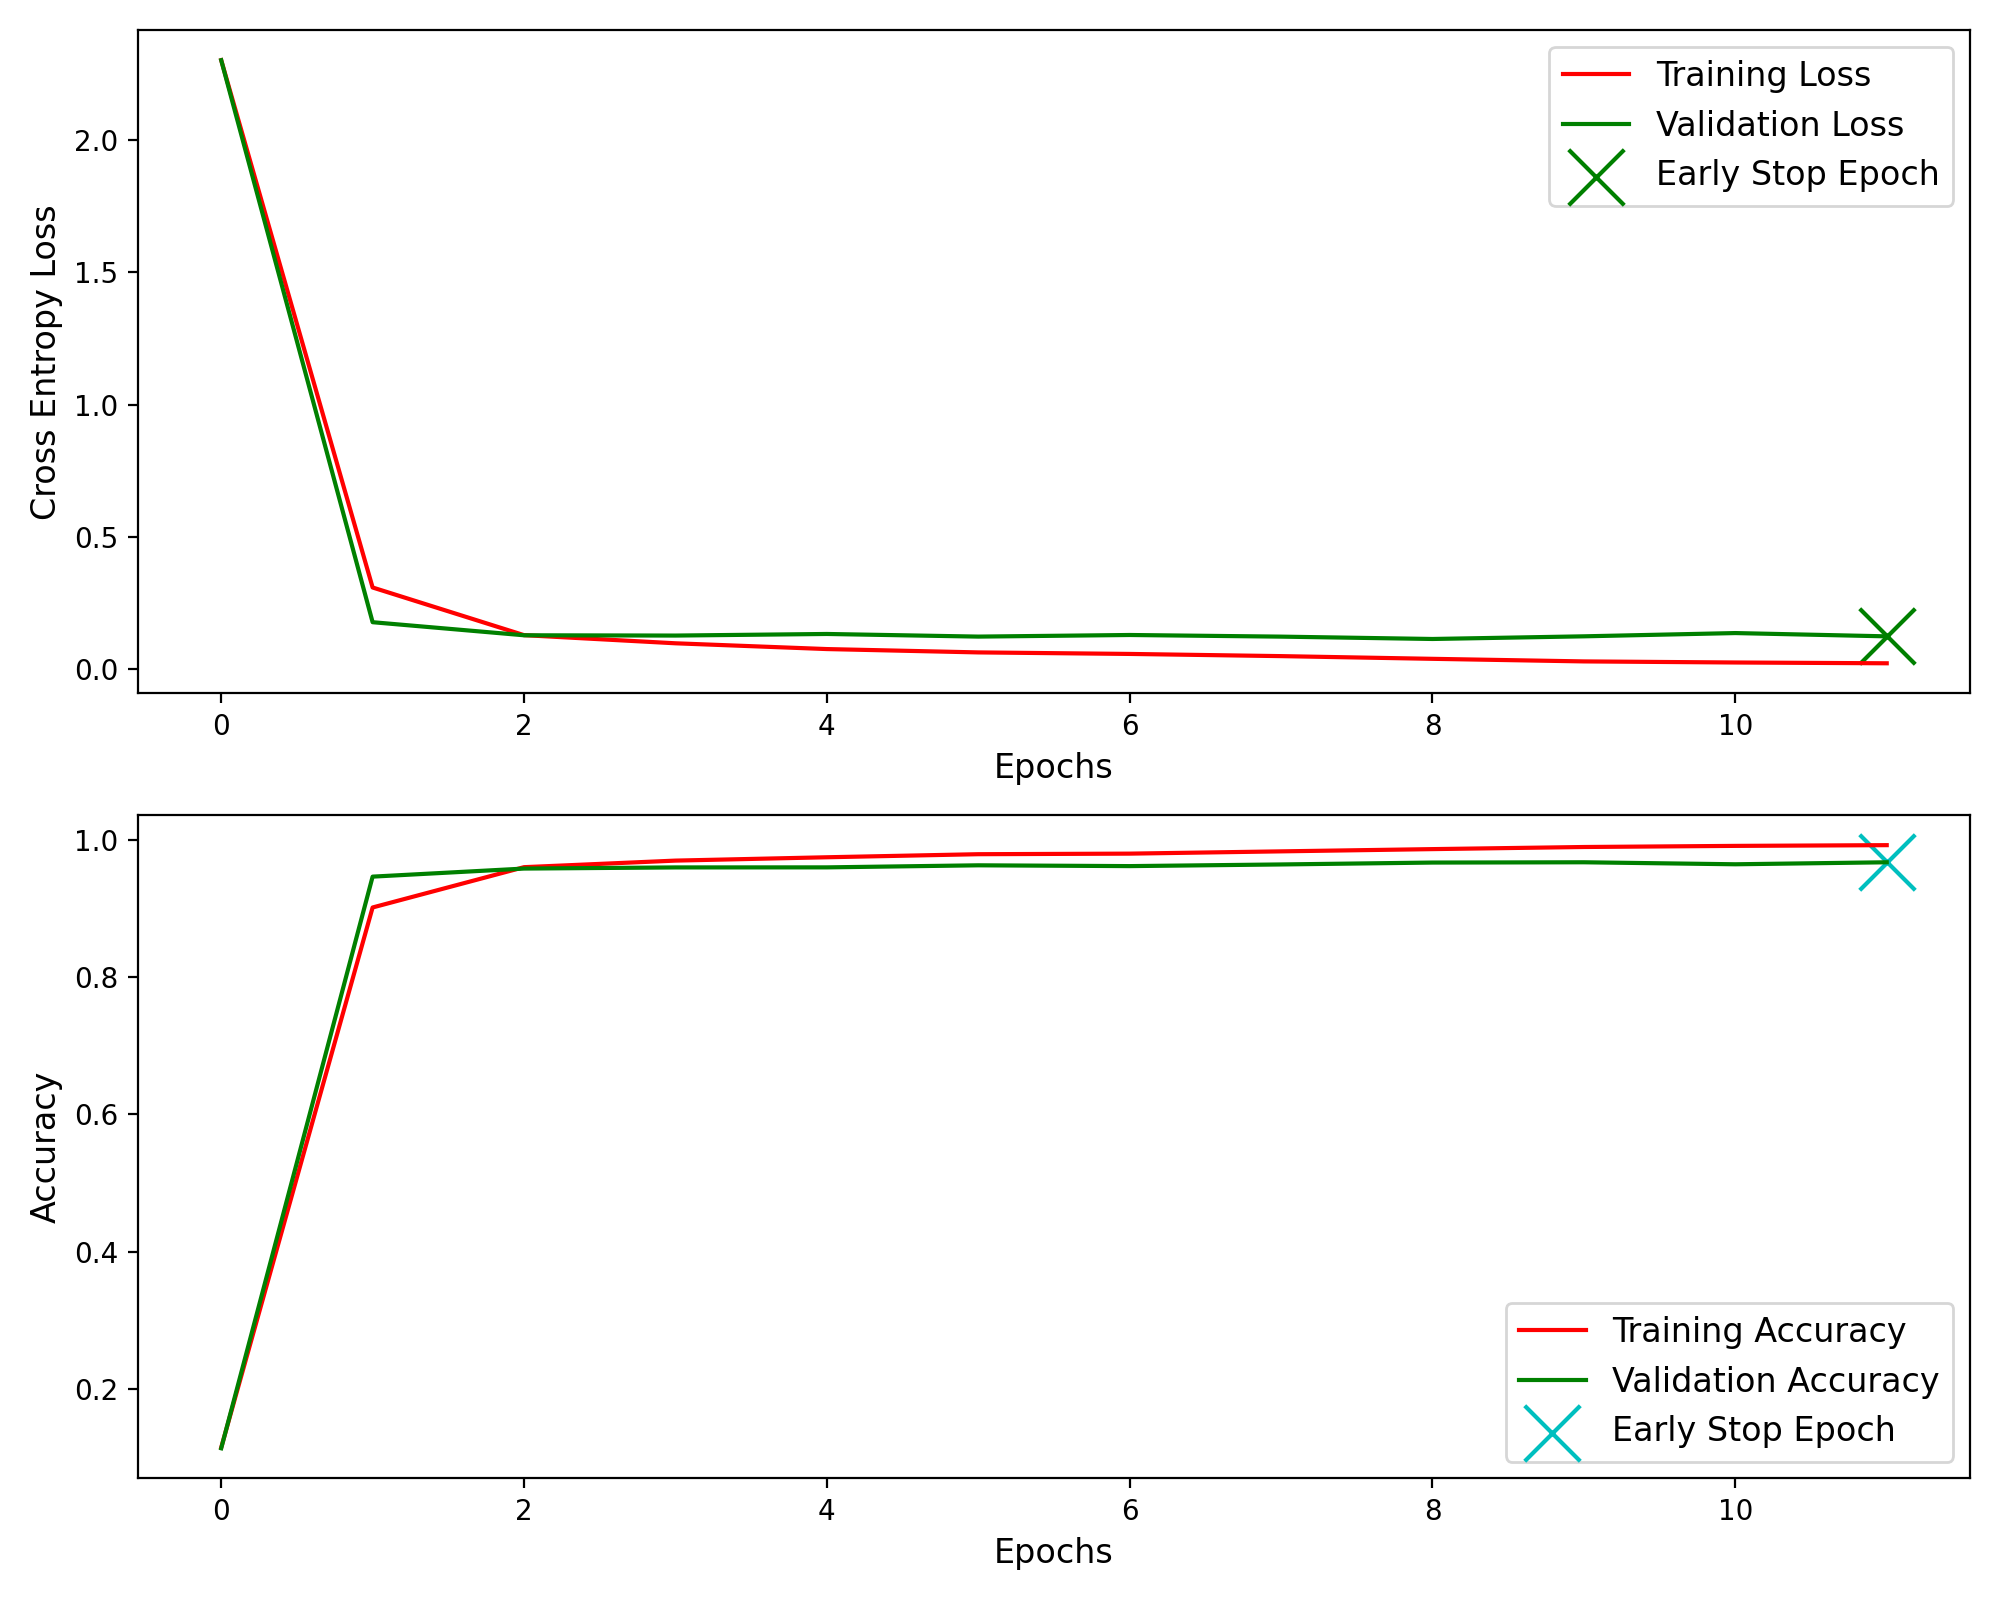
\includegraphics[width=1.0\textwidth]{./images/activation_tanh.png}
		\caption{Accuracy and Loss using $\tanh(x)$ activation}
		\label{fig:tanh}
	\end{subfigure}
	\begin{subfigure}{0.5\textwidth}
		\centering
		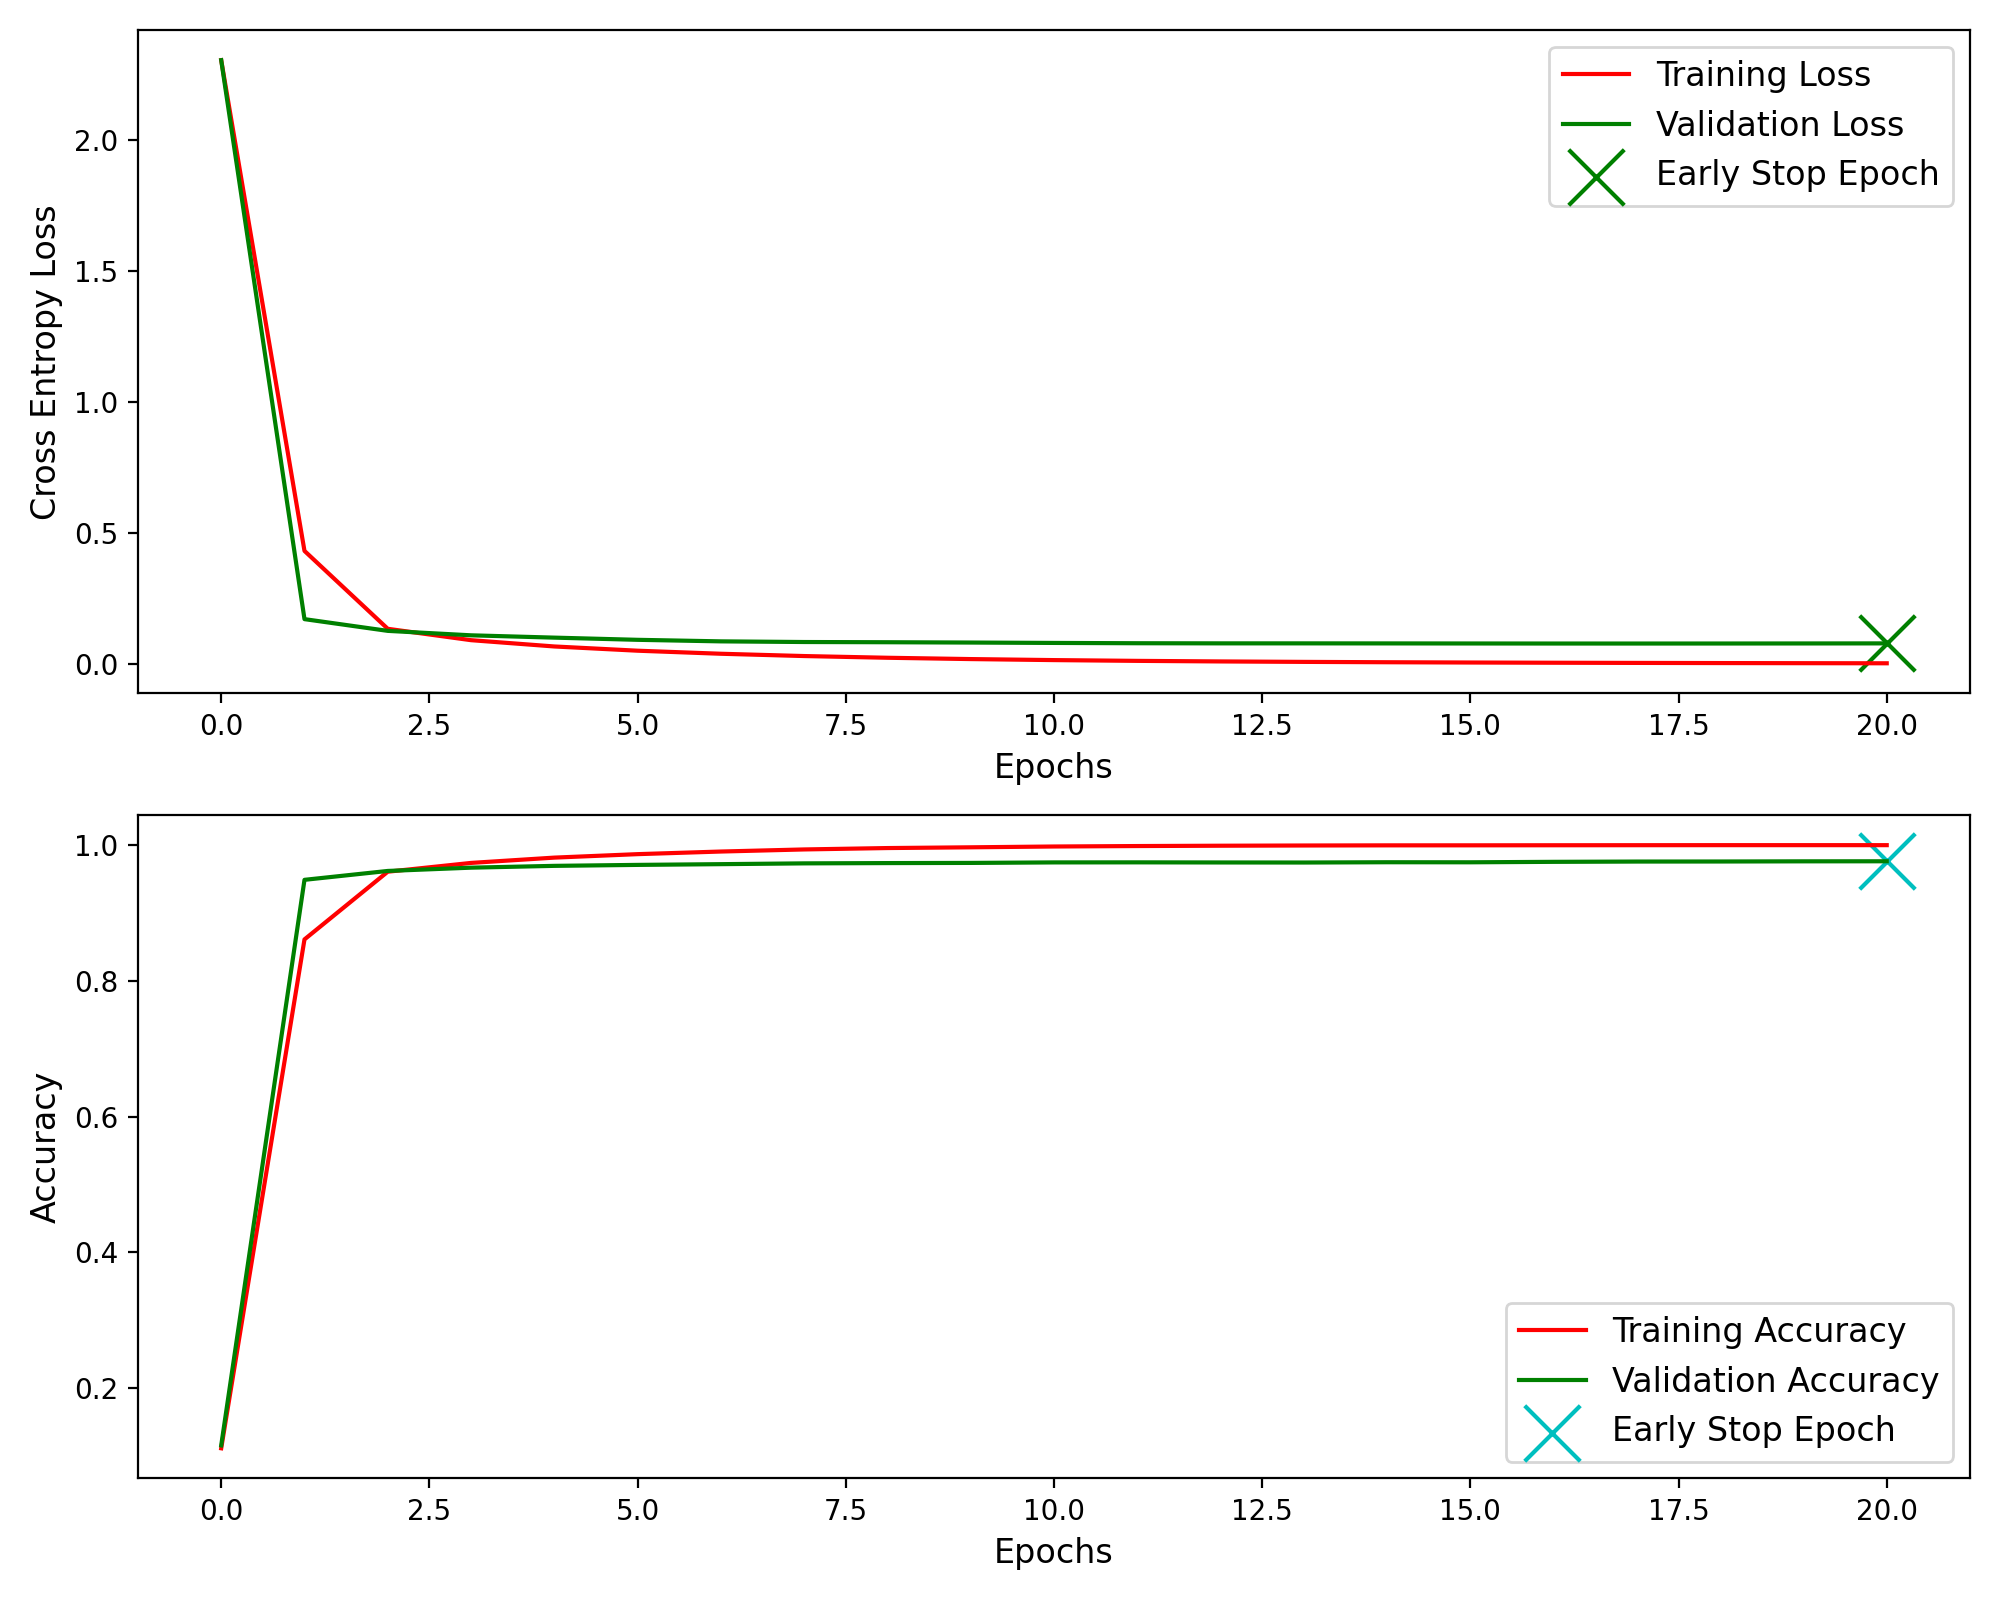
\includegraphics[width=1.0\textwidth]{./images/activation_sigmoid.png}
		\caption{Accuracy and Loss using $\texttt{sigmoid}(x)$ activation}
		\label{fig:sigmoid}
	\end{subfigure}
\end{figure}
\subsubsection{Sigmoid}


We get test accuracy of $97.66\%$ and a stopping epoch of $19$\cref{fig:sigmoid}.

\subsubsection{ReLU}

We get test accuracy of $95.61\%$ and a stopping epoch of $5$\cref{fig:relu}. The relatively
low performance and early stopping epoch suggests the learning rate is too high. If we set
$\alpha = 0.0001$, we get an accuracy of $97.56\%$ on the test data and stopping
epoch of $16$\cref{fig:relu2}.

\begin{figure}[H]
	\begin{subfigure}{0.5\textwidth}
		\centering
		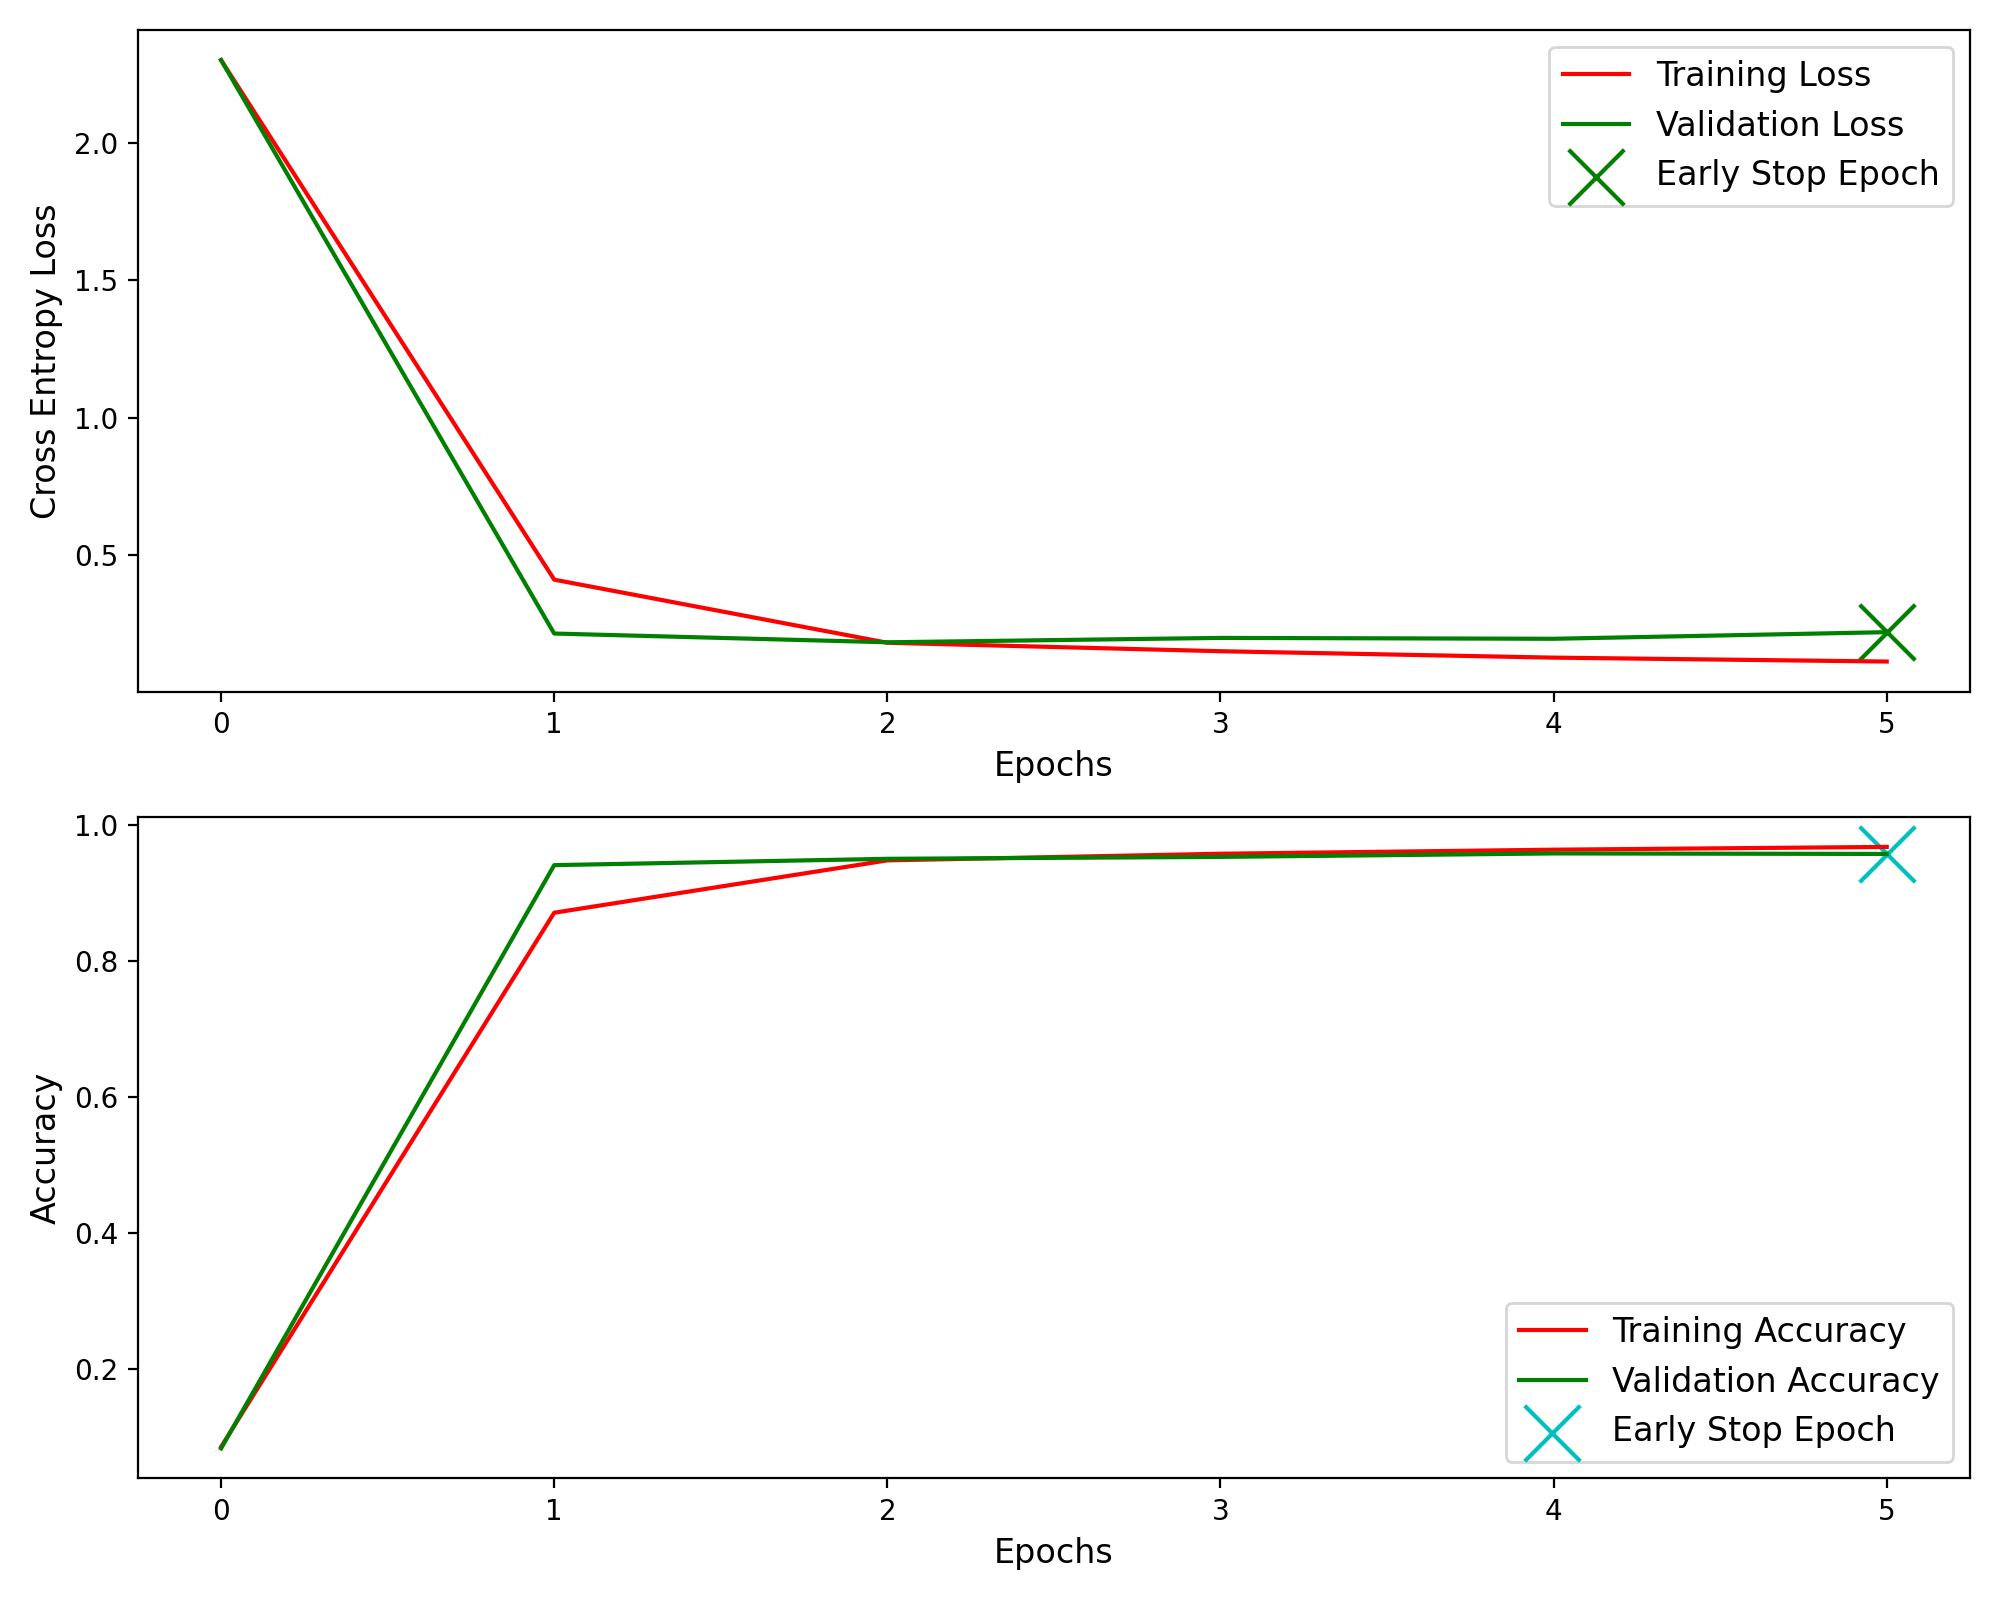
\includegraphics[width=1.0\textwidth]{./images/activation_relu.png}
		\caption{Accuracy and Loss using $\texttt{ReLU}(x)$ activation, $\alpha = 0.001$}
		\label{fig:relu}
	\end{subfigure}
	\begin{subfigure}{0.5\textwidth}
		\centering
		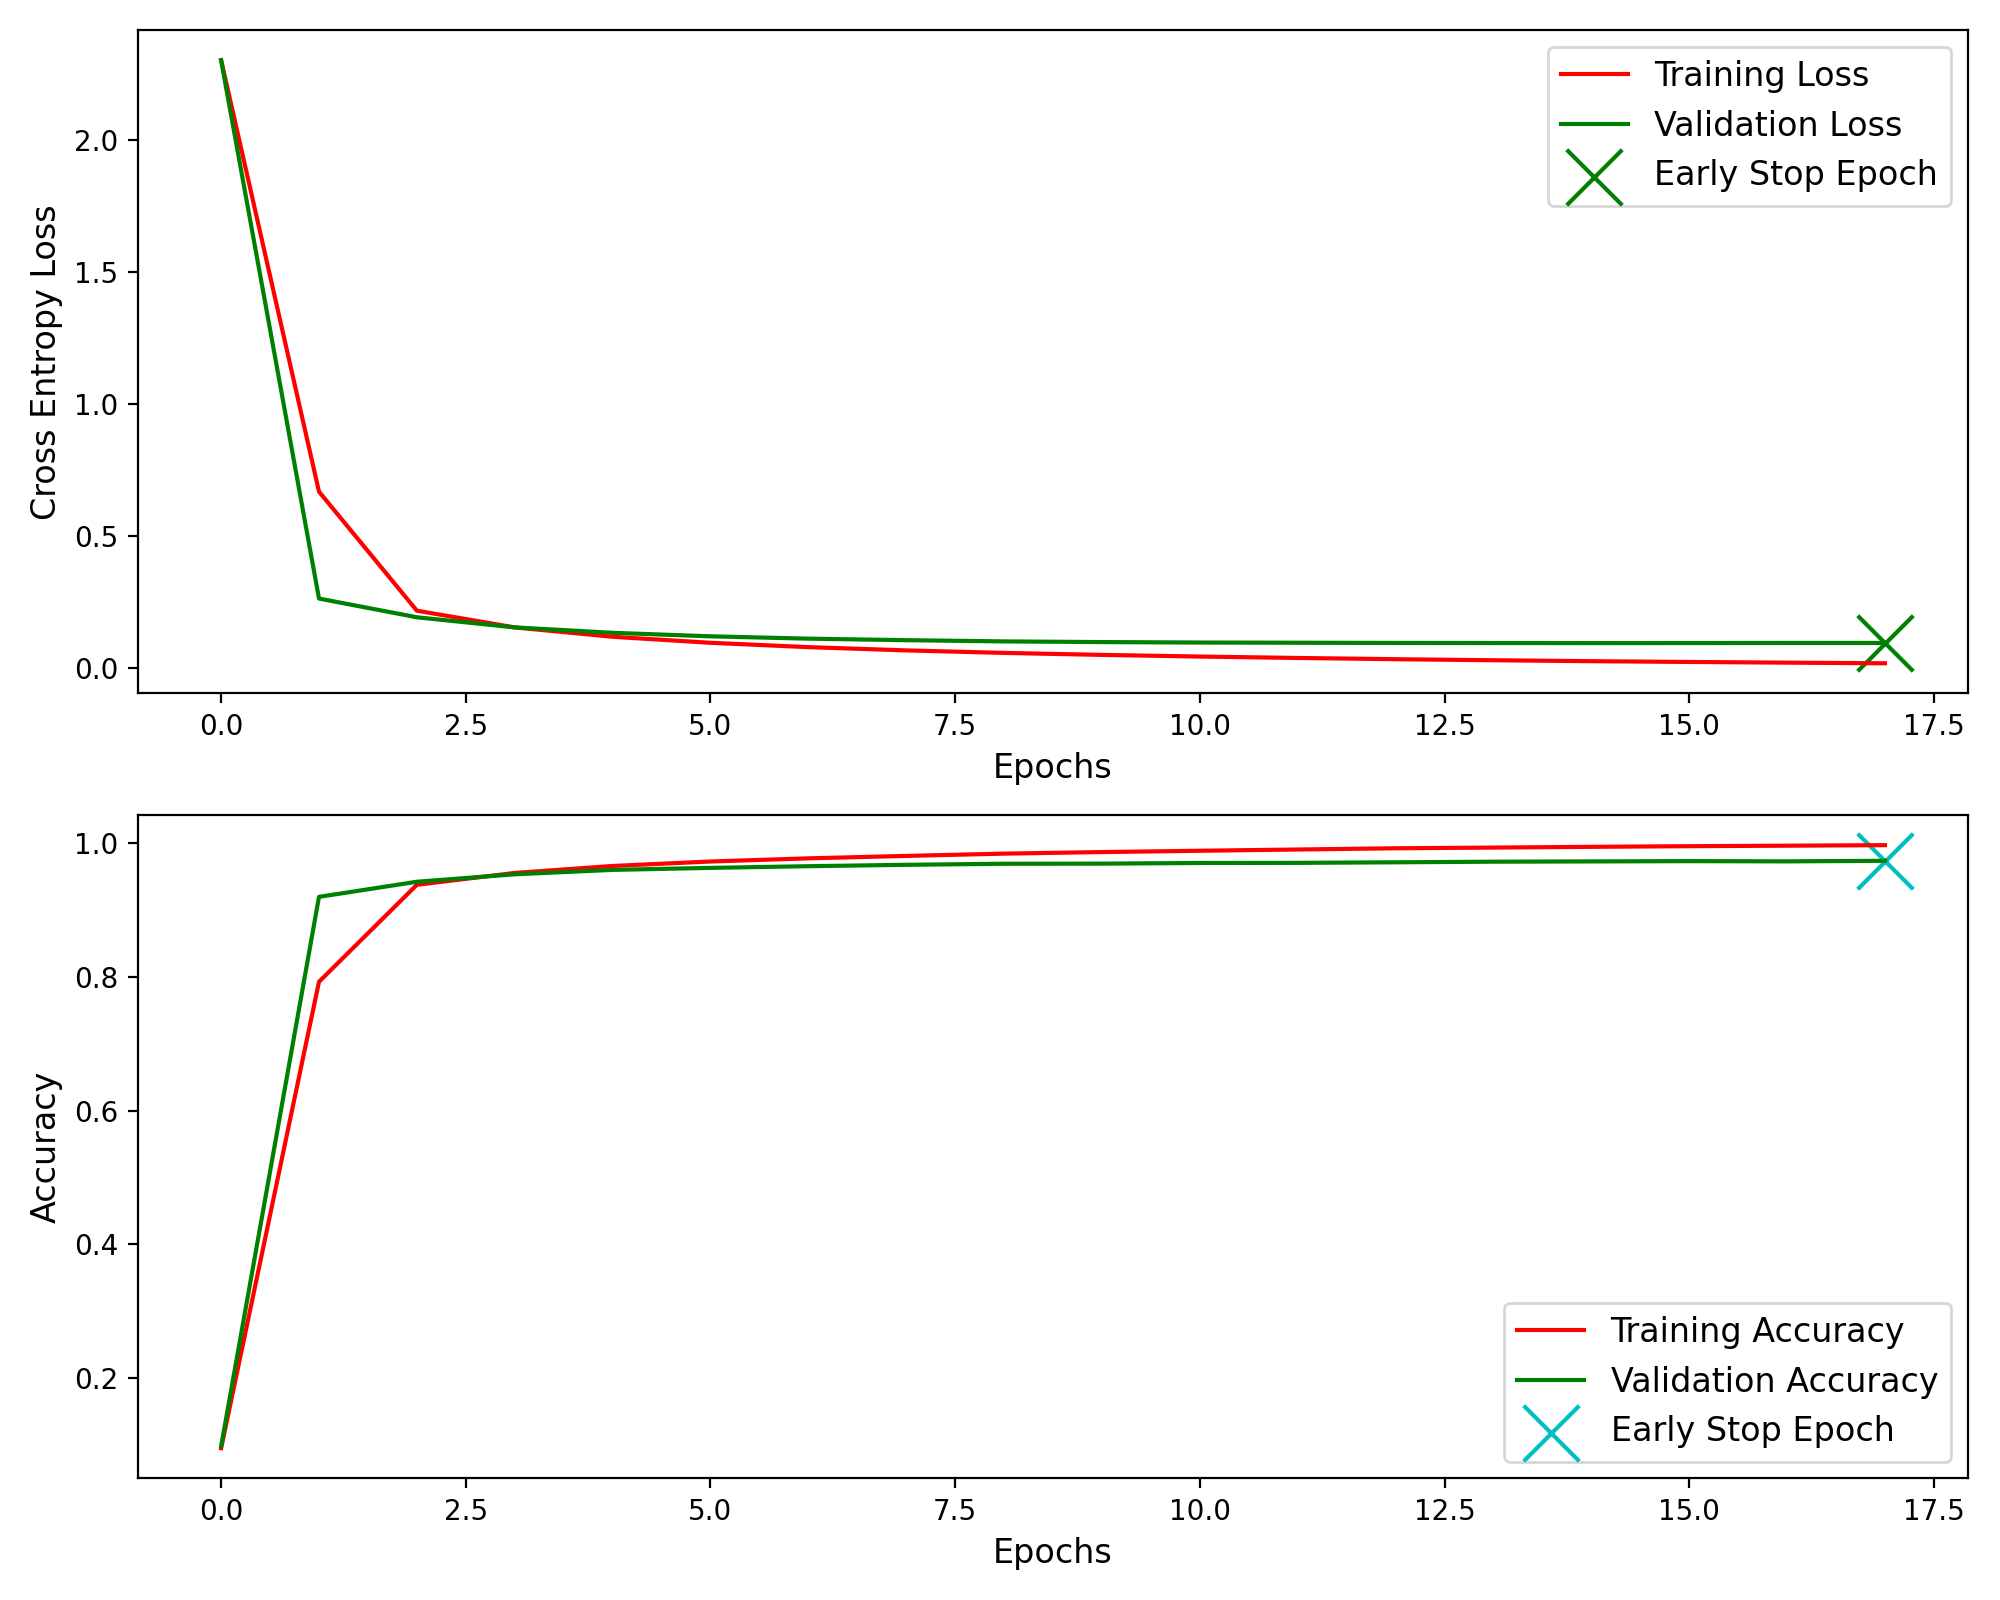
\includegraphics[width=1.0\textwidth]{./images/activation_relu2.png}
		\caption{Accuracy and Loss using $\texttt{ReLU}(x)$ activation, $\alpha = 0.0001$}
		\label{fig:relu2}
	\end{subfigure}
\end{figure}

\subsection{Observations}

With $\alpha = 0.001$ both sigmoid and tanh perform similarly on the test data, but
tanh converges much faster. ReLU performs fine, but poorly compared to the other two.
After seeing that ReLU was converging very fast, we tried reducing the learning rate
by a factor of 10. This brought ReLU's performance up to speed, but reduced its covergence time.

\begin{figure}[H]
	\centering
	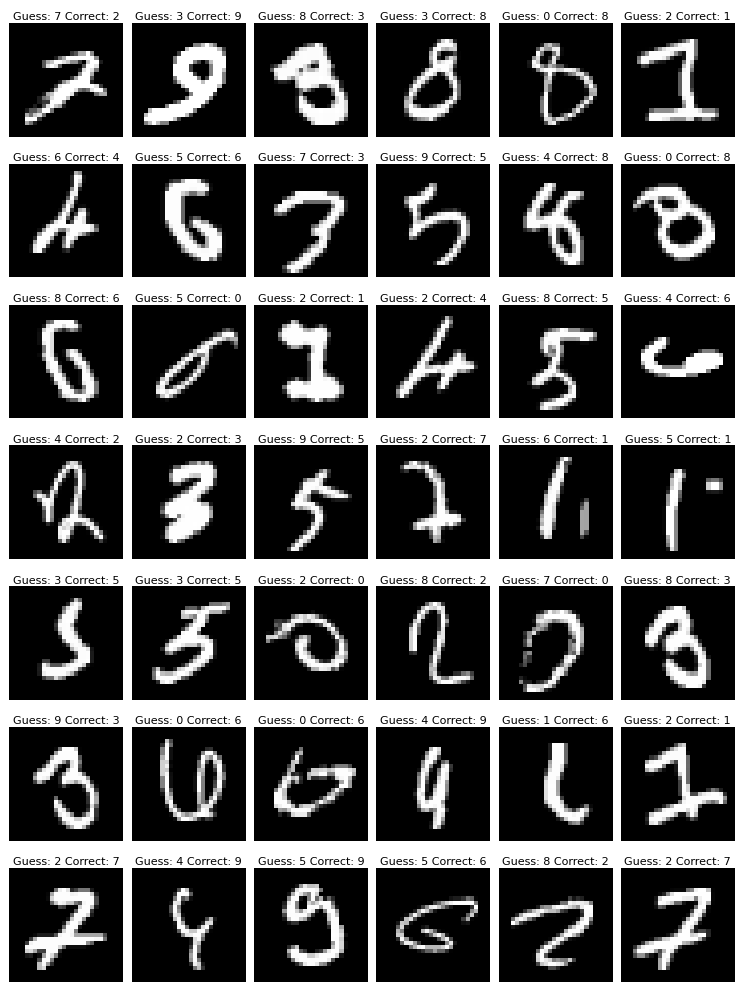
\includegraphics[width=0.8\textwidth]{./images/highest_loss_digits.png}
	\caption{Digits in the test set with the highest loss}
	\label{fig:highest_loss_digits}
\end{figure}


\begin{figure}[H]
	\centering
	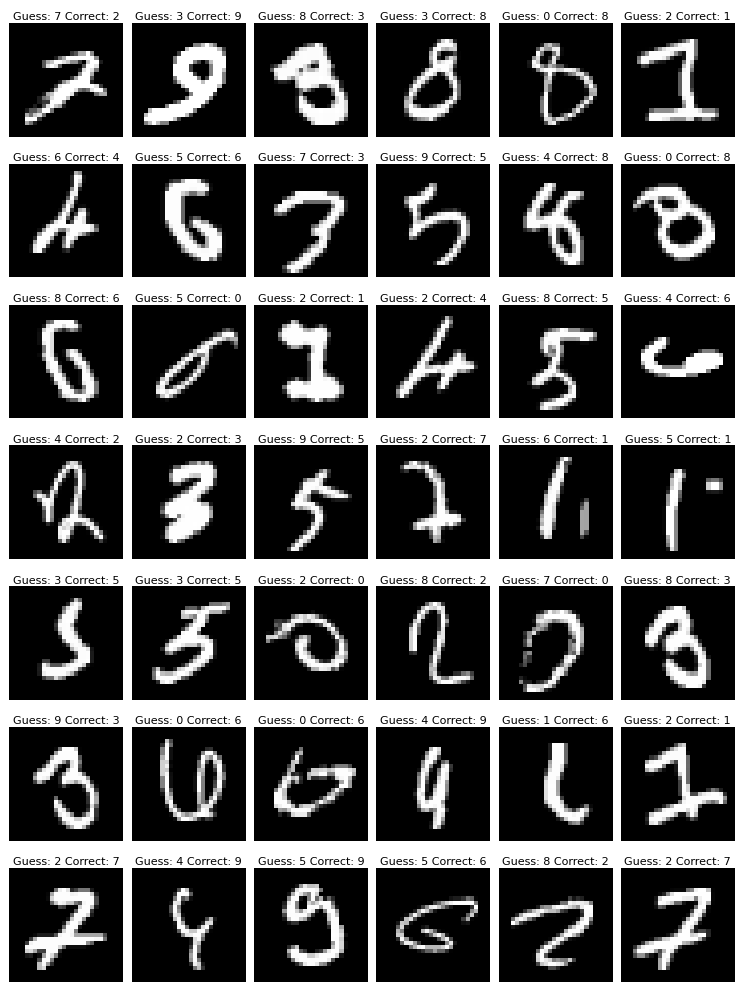
\includegraphics[width=1.0\textwidth]{./images/highest_loss_digits.png}
	\caption{Digits in the test set with the highest loss}
	\label{fig:highest_loss_digits}
\end{figure}

\section*{References}


References follow the acknowledgments in the camera-ready paper. Use unnumbered first-level heading for
the references. Any choice of citation style is acceptable as long as you are
consistent. It is permissible to reduce the font size to \verb+small+ (9 point)
when listing the references.
Note that the Reference section does not count towards the page limit.

\medskip


{
\small


[1] Alexander, J.A.\ \& Mozer, M.C.\ (1995) Template-based algorithms for
connectionist rule extraction. In G.\ Tesauro, D.S.\ Touretzky and T.K.\ Leen
(eds.), {\it Advances in Neural Information Processing Systems 7},
pp.\ 609--616. Cambridge, MA: MIT Press.


	[2] Bower, J.M.\ \& Beeman, D.\ (1995) {\it The Book of GENESIS: Exploring
		Realistic Neural Models with the GEneral NEural SImulation System.}  New York:
TELOS/Springer--Verlag.


[3] Hasselmo, M.E., Schnell, E.\ \& Barkai, E.\ (1995) Dynamics of learning and
recall at excitatory recurrent synapses and cholinergic modulation in rat
hippocampal region CA3. {\it Journal of Neuroscience} {\bf 15}(7):5249-5262.
}


\end{document}
